\chapter{Colisões (Opcional)}
\label{chap:colisaoopcional}
\vspace{-0.7cm}
%\let\clearpage\relax
\thispagestyle{empty}
\section{Introdução}

Neste experimento propomos um estudo de colisões entre dois corpos, que o aluno pode executar todo em casa. O sistema físico estudado é composto por duas moedas apoiadas sobre uma superfície lisa. Uma delas está inicialmente em repouso e a outra é lançada sobre ela, deslizando. Nosso foco é explorar quais grandezas se alteram e quais se conservam durante a colisão. Analisamos o momento linear e a energia mecânica das moedas individualmente e, muito importante, do sistema formado pelas duas juntas.

Agora em duas dimensões, a pergunta básica feita antes no seu experimento unidimensional sobre o momento linear total do sistema se divide em duas: Há conservação do momento linear total na direção $x$? Há conservação do momento linear total na direção $y$? A energia é uma grandeza escalar e continuamos perguntando: A energia mecânica total E do sistema se conserva na colisão estudada? 

Uma diferença fundamental entre este e o estudo que utilizou a filmagem do trilho de ar é a presença aqui de uma força atrito sobre cada moeda enquanto ela se desloca. Propomos explorar uma diferença qualitativa entre (i) as forças de atrito entre as moedas e a superfície e (ii) as forças de contato entre as moedas. As forças de contato, ditas {\it forças impulsivas}, são muito mais intensas que as forças de atrito, mas atuam apenas durante a colisão em si. O efeito das forças de atrito sobre as moedas no curto intervalo de tempo durante o qual elas interagem é muito pequeno: durante a colisão dominam as forças de contato. Assim, a discussão sobre conservação de momento e energia durante a colisão continua basicamente a mesma da situação sem atrito.

Este roteiro usa como exemplo o choque entre duas moedas de 1 Real, e indica dois caminhos para a análise da colisão. Use o exemplo fornecido para se ambientar com o estudo de colisões, mas não se preocupe em reproduzir as trajetórias mostradas ou em usar também moedas de 1 Real. Lance uma de suas moedas em direção à outra, e analise o resultado da colisão entre as duas. As sugestões para registrar o movimento e analisar os dados estão nas próximas seções. Na primeira sugestão para análise, a informação sobre a colisão vem de medidas da distância percorrida depois da colisão por cada uma das moedas \cite{Galante2020} e do ângulo entre essas duas trajetórias.  Na segunda, são feitas medidas diretas de posição em função do tempo com uma taxa alta o suficiente para revelar o caráter impulsivo das forças de contato~\cite{deJesus2016}
%\cite{deJesus2016}.

Neste experimento você tem liberdade na organização de um relatório a ser encaminhado ao professor. Note que é importante que seu texto tenha suporte em uma ou mais imagens relativas à sua montagem experimental e às análises gráfica e/ou numérica do movimento.


%o movimento depois da colisão até as duas moedas atingirem o repouso, depois de dissipar toda sua energia cinética em decorrência das forças de atrito.\cite{Galante2020}. Na segunda, fazemos medidas diretas de posição em função do tempo 

%a informação é obtida a partir dos traços defi  
%analise o movimento até as duas moedas atingirem o repouso depois de dissipar toda sua energia cinética em decorrência das forças de atrito.

%Sugerimos duas estratégias para a análise de conservação de momento linear. Na primeira se restrinja a poucos quadros antes e depois da colisão. Na segunda, analise o movimento até as duas moedas atingirem o repouso depois de dissipar toda sua energia cinética em decorrência das forças de atrito.

%Por fim, seguem algumas observações sobre sua empreitada. Capriche na sua montagem experimental, mas não seja tão perfeccionista que acabe não fazendo o experimento do início ao fim. Também não se preocupe se você não consegue entender o que está por trás de cada detalhe do movimento. Você pode aprender bastante tentando modelar o sistema físico estudado em sua casa à partir do que está aprendendo em suas aulas teóricas. Mas repare como é também importante  descrever suas observações e as condições nas quais elas são feitas, e ressaltar pontos interessantes entre seus resultados.

%Na tomada de dados o movimento é gravado em um filme. A variação das posições dos corpos é analisada posteriormente. Programas de computador como aquele já utilizado no experimento anterior, o Tracker, são bastate úteis nessa análise.

%Para essa segunda parte, apontamos ainda uma versão simplificada do experimento que, fazendo suposiões sobre o atrito, permite fazer um teste da conservação de momento linear em uma colisão, mesmo sem celular ou computador.

\section{Procedimento experimental}

\subsection{Realização das medidas}

O procedimento para realizar a colisão é simples: procure em sua casa uma superfície plana e lisa sobre a qual as moedas possam deslizar com o menor atrito possível. Dê um peteleco em uma das moedas, lançando-a em direção à outra. Teste diferentes superfícies. No caso mostrado como exemplo neste roteiro foi usada uma superfície de fórmica. Utilize um aparelho celular para filmar todo o experimento, desde o instante inicial do movimento até o repouso final das moedas.

Experimente diferentes velocidades iniciais do objeto incidente. Se a velocidade for muito baixa, o atrito fará a moeda incidente parar muito rápido, inviabilizando o experimento. Se a velocidade for alta demais, o celular não irá conseguir capturar imagens com uma taxa alta o suficiente para estudar o movimento. Fazer a filmagem no modo em câmera lenta pode ajudar. É comum que os celulares façam filmagens em seu modo padrão com taxa de 30 quadros por segundo (ou {\it frames per second} - fps). Possívelmente seu celular é capaz de fazer a filmagem em um modo em câmera lenta com 120 fps ou mais. Se esse for o caso, aproveite essa opção, mas certifique-se de que seu filme não seja comprimido antes da análise. Se usar 30 fps, faça o filme com muita luz, de preferência ao Sol, evitando assim imagens borradas.

Uma vantagem no uso das moedas é que suas massas podem ser descobertas com uma pesquisa na internet. O diâmetro das moedas também é informação de fácil obtenção {\it online}, e pode ser usada para calibrar as distâncias na análise dos dados. Use duas moedas iguais para que as forças de atrito sejam iguais.

\subsection{Análise das imagens}

\begin{figure}
\centering
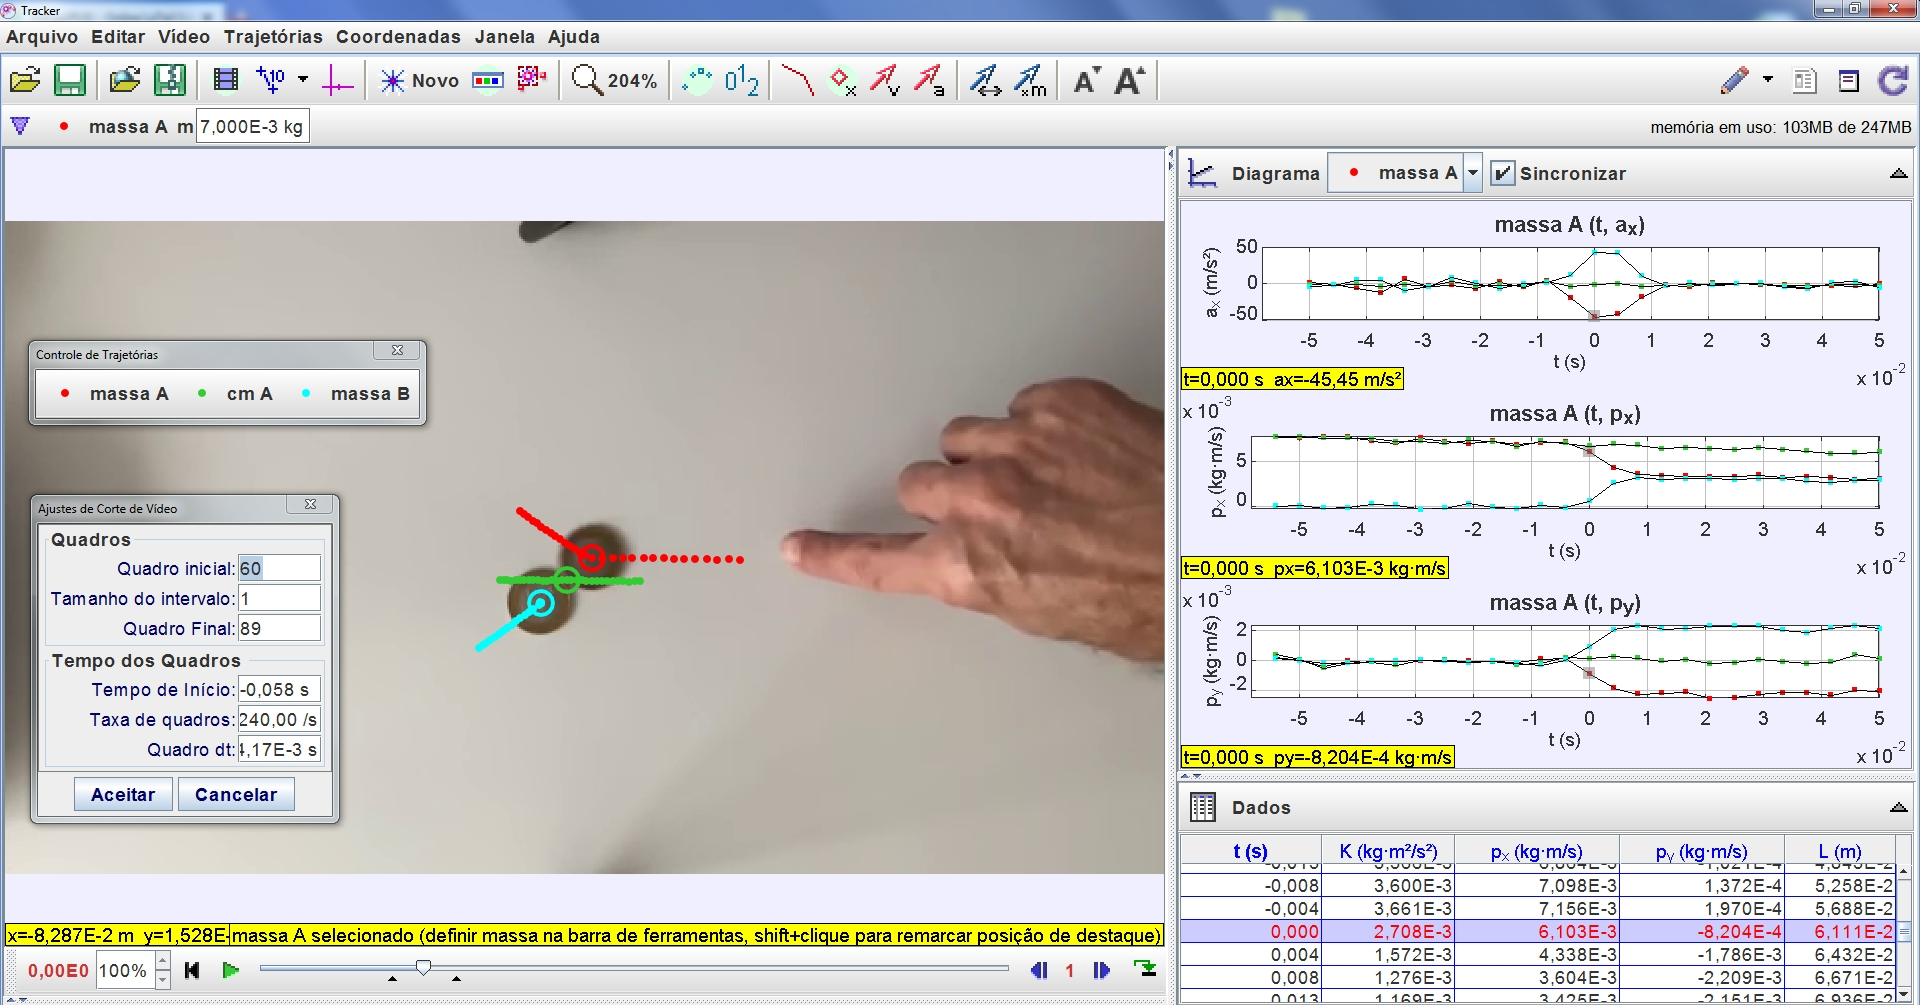
\includegraphics[width=0.7\columnwidth]{Figuras_exp4/figcolisaomoedas1.jpg}
\caption{\label{fig:figcolisaomoedas1} Tela típica de análise com o programa Tracker.}
\end{figure}

Os dois métodos sugeridos para análise da colisão baseiam-se em medidas de posição sobre imagens registradas em função do tempo. O programa Tracker (Apêndice~\ref{sec:tracker}), usado anteriormente no Experimento 3 e agora no 4, é uma ferramenta interessante para uso nos dois métodos. 

A partir de suas medições para as posições de cada um dos corpos, e de informação sobre suas massas, você poderá obter também a evolução da posição do centro de massa do sistema. Note que as forças de interação entre os dois objetos são internas ao sistema. Assim, não influenciam o movimento do centro de massa (CM), que deve ser mais simples que o movimento de cada um dos corpos. Analise o comportamento do CM do sistema antes, durante e depois da colisão.

Depois de importar seu filme para o Tracker, entre no programa com a informação sobre a taxa de quadros por segundo da sua filmagem. Dê um ``zoom'' nas suas imagens para marcar melhor as posições dos centros de massa de cada moeda. O próprio programa calcula e representa a posição do CM do sistema.

Com o programa Tracker você pode ainda gerar facilmente gráficos de velocidade, aceleração, momento linear, energia e outros. 
A Figura~\ref{fig:figcolisaomoedas1} mostra uma tela típica do Tracker em uma análise desse tipo, na qual os gráficos escolhidos são feitos automaticamente à medida que os pontos são marcados sobre a imagem. O programa utiliza para isso derivação numérica, mas você não precisa aqui se preocupar com os detalhes desse procedimento matemático. Se estiver curioso, pode ver na apostila um exemplo de derivação numérica na seção sobre  “Determinação da velocidade instantânea". Os gráficos de aceleração de cada um dos corpos são úteis para você entender o caráter impulsivo das forças de interação na colisão. Você pode também construir seus gráficos à mão ou utilizando um programa específico para essa função (consulte o Capítulo~\ref{chap:minquad} “representações gráficas"  da Apostila). 


%Sugerimos duas estratégias para a análise de conservação de momento linear. 

%Na primeira se restrinje a poucos quadros antes e depois da colisão. Na segunda, analise o movimento até as duas moedas atingirem o repouso depois de dissipar toda sua energia cinética em decorrência das forças de atrito.

 
\section{Exemplo de resultados e análise}


\subsection{ Medidas do traço de posição até o repouso das moedas}

\begin{figure*}
\centering
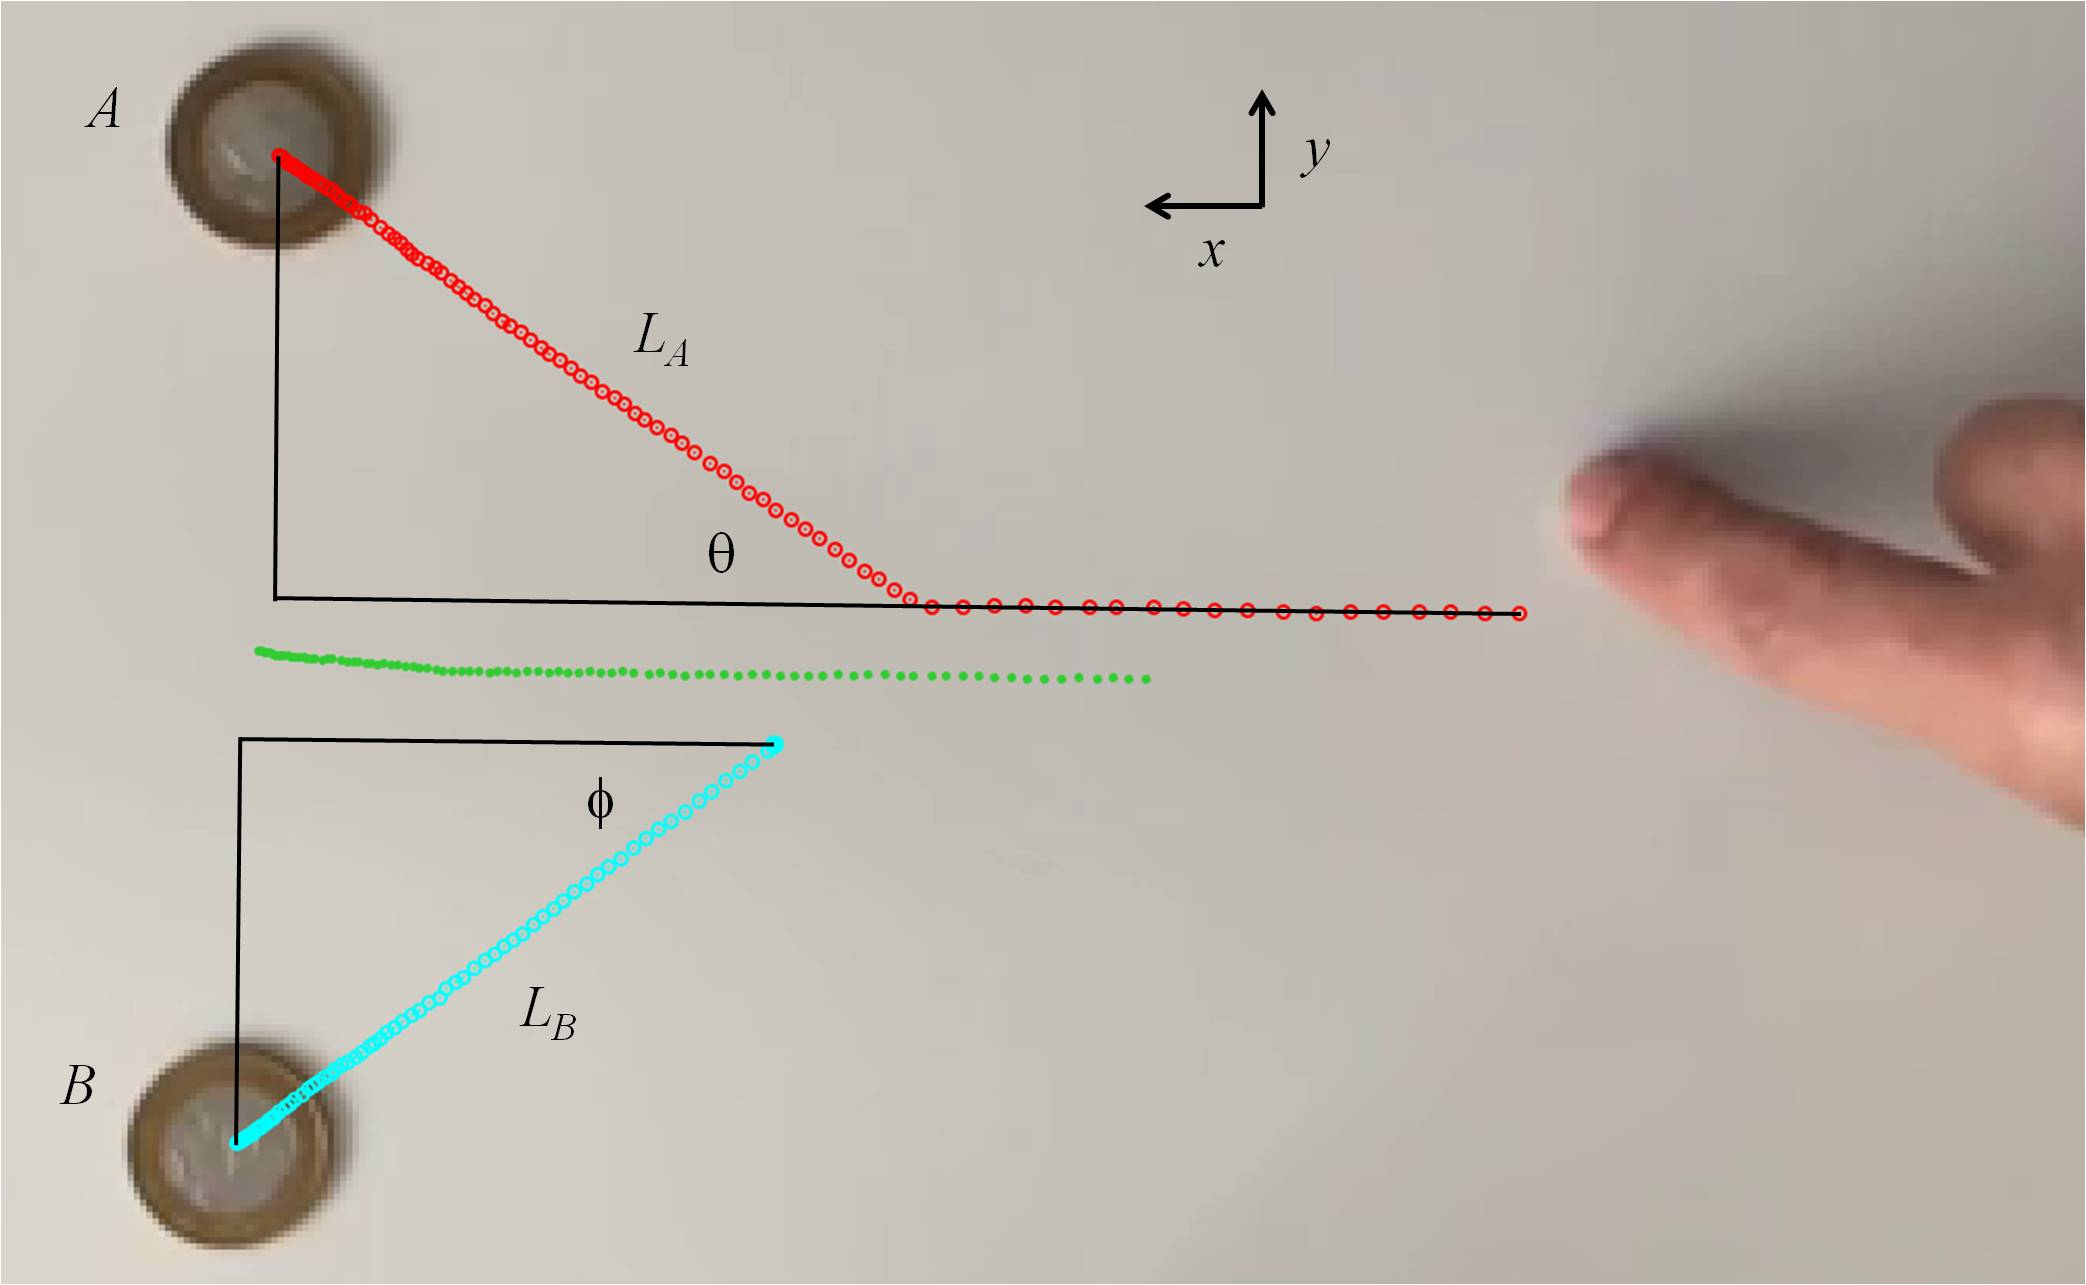
\includegraphics[width=0.5\columnwidth]{Figuras_exp4/figcolisaomoedas3.jpg}
\caption{\label{fig:figcolisaomoedas3} Moedas em suas posições finais e marcações de suas trajetórias (CM em verde).}
\end{figure*}

A primeira estratégia que indicamos para testar a conservação de momento linear na colisão de duas moedas, na presença de atrito, foi sugerida recentemente por Galante e Gnesi~\cite{Galante2020}.

Eles chamam a atenção para similaridades dela com métodos calorimétricos com os quais se mede o momento de uma partícula sub atômica a partir de um rastro que ela deixa em um detetor. Na versão simplificada com moedas colidindo, é assumido que a força de atrito é constante e o teorema trabalho-energia cinética é usado para estimar os módulos dos momentos lineares das duas moedas depois da colisão. Temos assim para cada moeda a relação entre o módulo de seu momento $p$ logo após a colisão e o alcance $L$ até parar:
\begin{equation}
\frac{p^2}{2m} = F_{at}~L, 
\end{equation}
onde $F_{at}$ é o módulo da força de atrito e $m$ é a massa da partícula. Se as moedas são iguais, $m$ e $F_{at}$ são iguais para as duas, e obtemos (ver Figura \ref{fig:figcolisaomoedas3}):
\begin{equation}
\frac{p_A}{p_B} = \sqrt{\frac{L_A}{L_B}}.
\end{equation}
Tomando a direção de incidência da moeda A em $x$, e considerando a moeda B inicialmente parada, a componente do momento linear total em $y$ antes da colisão é zero. Logo, devemos ter depois da colisão as componentes ${\text p}_{Ay}$ e ${\text p}_{By}$ com mesmo módulo e sinais contrários e, portanto, a razão entre elas deve ser igual a -1. Para testar essa hipótese, precisamos medir também os ângulos entre os momentos finais e a direção de incidência da moeda projétil, a fim de determinar 
\begin{equation}
\frac{{\text p}_{Ay}}{{\text p}_{By}} = -\frac{p_A~{\text sen}(\theta)}{p_B~{\text sen}(\phi)} = - \sqrt{\frac{L_A}{L_B}}~\frac{{\text sen}(\theta)}{{\text sen}(\phi)}.
\end{equation}

A partir da Figura \ref{fig:figcolisaomoedas3}, na qual foram marcadas as posições das moedas até elas pararem, obtemos 
$L_A=(0,111 \pm 0,003)$~m, 
${\text sen}(\theta)=(0,57 \pm 0,02)$, 
$L_B=(0,091 \pm 0,003)$~m, 
e ${\text sen}(\phi)=(0,60 \pm 0,02)$. 
Assim, obtemos experimentalmente, depois da colisão:
\begin{equation}
\frac{{\text p}_{Ay}} {{\text p}_{By}} = - 1,05 \pm 0,05.
\end{equation}
Este resultado mostra que a soma das componentes ${\text p}_{Ay}$ e ${\text p}_{By}$, dentro do erro experimental, permanece igual a zero depois da colisão. Verificamos assim que a componente $y$ do momento linear total se conservou nesse experimento.

A variação percentual de energia na colisão pode ser expressa como (dedução no Apêndice deste roteiro):
\begin{equation}
\frac{E_f - E_i}{E_i} = \frac{-1}{1+ \displaystyle {\frac{\sqrt{\frac{L_A}{L_B}}+\sqrt{\frac{L_B}{L_A}}}{2~ \cos(\theta+\phi)}}}.
\label{eqE}
\end{equation}
A Eq. \ref{eqE} mostra que se não houvesse perda de energia cinética na colisão, teríamos um ângulo entre os vetores momento final dos dois corpos $\theta+\phi=90^{\degree}$. No entanto,
da Figura \ref{fig:figcolisaomoedas3} temos $\theta+\phi= 72^{\degree}$ e $L_A/L_B=1,2$. Nesse caso, substituindo valores na Eq. \ref{eqE}, determinamos uma diminuição, devida à colisão, de $24\%$ na energia cinética total do sistema. A colisão é, portanto, inelástica. 

Note que você pode filmar a colisão, como feito aqui, mas isso não é essencial. No experimento original de Galante e Gnesi eles usam apenas moedas, lápis, papel, e régua. O preço da simplicidade neste método é assumir que a força de atrito é constante e igual, em módulo, para as duas moedas. 


\subsection{ Medidas de posição durante curto intervalo de tempo}

\begin{figure*}
\centering
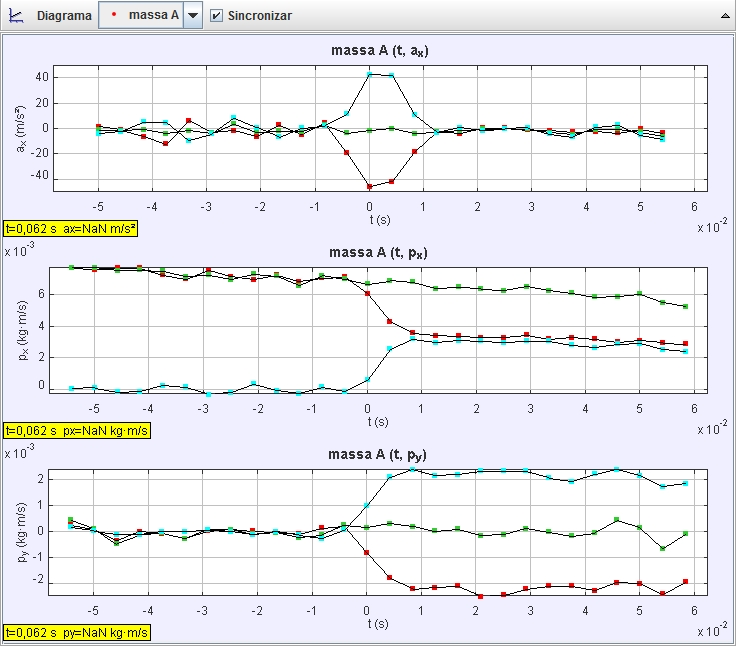
\includegraphics[width=0.7\columnwidth]{Figuras_exp4/figcolisaomoedas2.jpg}
\caption{\label{fig:figcolisaomoedas2} Gráficos de a$_x$, p$_x$ e p$_y$ em função do tempo. Moeda A em vermelho, moeda B em azul e  centro de massa do sistema moeda A mais moeda B em verde. }
\end{figure*}
Analisando apenas um curto intervalo de tempo antes e depois da colisão, o efeitos da força de atrito nas variações de momento linear em cada moeda serão pequenos em relação aos efeitos da força de contato entre as moedas. Os gráficos da Figura~\ref{fig:figcolisaomoedas1} estão reproduzidos com destaque na Figura~\ref{fig:figcolisaomoedas2}: aceleração na direção $x$ (direção dada pela moeda incidente), componente do momento linear na direção $x$, e componente do momento linear na direção $y$. Em cada gráfico é feita uma comparação dos valores associados à moeda A (em vermelho), à moeda B (em azul), e ao centro de massa do sistema moeda A mais moeda B (em verde). O gráfico da aceleração mostra no momento da colisão um pico para a moeda B e um pico invertido bastante similar para a moeda A. Esses picos refletem as forças de contato durante a colisão. Ainda no mesmo gráfico, vemos que a duração da colisão é de cerca de um centésimo de segundo. Para efeito de comparação, perceba que a aceleração de cada moeda chega, durante a colisão, a cerca de quatro vezes o valor da aceleração da gravidade, mas cai rapidamente quando apenas a força de atrito está presente. 

É possível demonstrar que o produto da massa pela área de cada um dos picos é igual à variação do momento linear. Assim, picos simétricos no gráfico de aceleração na Figura~\ref{fig:figcolisaomoedas2} demonstram a conservação do momento linear total do sistema, neste caso na direção $x$. Note que a aceleração do centro de massa é próxima de zero antes, durante e depois da colisão. A conservação de momento linear em $x$ e em $y$ durante a colisão pode ser vista também diretamente nos dois últimos gráficos da Figura~\ref{fig:figcolisaomoedas2}, ligeiramente mascarada por uma pequena e lenta variação do momento linear total devida às forças de atrito, que são externas ao sistema moeda A mais moeda B.


%Nesta segunda parte o aluno decide qual será sua montagem experimental feita em casa, filma a colisão com o celular, e faz a análise do movimento usando o programa Tracker, já utilizado anteriormante no curso.



%A seguir apresentamos uma sugestão de experimento a ser feito em casa: colisão bidimensional entre duas moedas no plano. Apresentamos imagens e um de conjunto de dados para você se familiarizar, mas lembre-se: o importante aqui é você obter e analisar seus prórios dados experimentais. Outras sugestões, como colisão entre bolinhas de gude e colisão entre blocos de gelo, estão em um arquivo separado na homepage da disciplina. Você pode escolher uma das três para fazer na sua casa ou ainda desenvolver uma ideia nova, sem perder de vista que nosso foco é o estudo do comportamento do momento linear total em colisões. 




%Por fim, seguem algumas observações sobre sua empreitada. Capriche na sua montagem experimental, mas não seja tão perfeccionista que acabe não fazendo o experimento do início ao fim. Também não se preocupe se você não consegue entender o que está por trás de cada detalhe do movimento. Você pode aprender bastante tentando modelar o sistema físico estudado em sua casa à partir do que está aprendendo em suas aulas teóricas. Mas repare como é também importante  descrever suas observações e as condições nas quais elas são feitas, e ressaltar pontos interessantes entre seus resultados.




%\thispagestyle{plain}